
%\chapter{Project's Objectives and Specification}
 \chapter{Obiective și specificații}
\label{cap:obiective-specificatii}

%Acest capitol conține descrierea detaliată a temei de cercetare propriu-zise, formulată exact, cu obiective clare și specificații, pe 2-3 pagini și eventuale figuri explicative. Titlul nu e neapărat impus și, de asemenea, capitolul poate fi inclus ca subcapitol în Capitolul~\ref{cap:Introducere}, dacă se potrivește.
%
%Reprezintă cca. 5--10\% din lucrare.

Acest capitol prezintă obiectivele lucrării, motivând deciziile luate în implementarea sistemului, specificațiile sistemului, cerințele funcționale și nonfunctionale necesare implementării sistemului. 

%\section{Objectives}
 \section{Obiective}
%
%Obiectivele proiectului sunt lucrurile care se dorește a fi realizate, ca urmare a abordării temei lucrării de licență. În general numărul de obiective este proporțional cu timpul de care dispunem. Exemple generice:
%\begin{enumerate}
%  \item Analiza critică a soluțiilor existente pentru problema abordată și identificarea posibile limitări ale acestora.
%  \item Propunerea unor soluții la (o parte) din problemele identificate. 
%  \item Implementarea soluției și validarea ei
%  \item Identificarea unor teme de dezvoltare și cercetare ulterioare
%  \item \dots
%\end{enumerate}
Elaborarea unor măsuri de securitate împotriva anumitor tipuri de atacuri sau dezvoltarea unei logici de filtrare a clienților serviți de către aplicație este posibilă și în partea de implementare a serverului, ceea ce ar putea oferi și o eventuală creștere în performanțele aplicației, eliminând astfel posibile interceptări suplimentare și validări ale traficului. Însă o astfel de implementare presupune o arhitectură mult mai complexă pentru partea de server și individual cunoștințe avansate despre securitate, posibilele vulnerabilități la care acesta poate să fie predispus, precum și modalități de combatere ale acestora.  
  
O soluție mult mai simplă la această problemă este folosirea unui modul care să implementeze aceste funcționalități separat. Mare parte din produsele de pe piață, ce îndeplinesc aceste caracteristici sunt destul de scumpe și nu oferă foarte multă libertate din punctul de vedere al configurări securității dorite de către utilizator asupra produsului sau. În cazul IP-urilor blocate, multe aplicații nu oferă libertatea utilizatorilor de a edita listele de referință ale detecțiilor, acestea fiind actualizate automat conform unor date interne, iar eventualele abateri de la aceste reguli se realizează prin adăugarea de excepții. În cea ce privește validarea request-urilor primite de la clienți, mare parte din aceste sisteme nu oferă o protecție configurabilă. Cum s-a precizat mai sus, acest tip de sisteme pot să introducă mici întârzieri datorate validărilor suplimentare asupra request-urilor primite de la clienții produsului, însă în unele cazuri anumite validări sunt făcute inutil întrucât produsele respective neputând să prezinte vulnerabilități de acel fel. 

 \textit{\thesistitle}  are obiectivul de a oferi o componentă gratuită cât mai ușor de integrat și de configurat de către utilizator după preferințele produsului sau, care să facilizeze o protecție cât mai eficientă cu suport pentru îmbunătățiri. Sistemul trebuie să fie ușor de instalat și de configurat, oferindu-i utilizatorului o interfață clară, sugestivă și ușor de folosit prin care să interacționeze cu acesta. Detecțiile sistemului trebuie să fie selectabile, utilizatorul putând alege în momentul pornirii sistemului ce vulnerabilități să fie tratate de acesta. Lista IP-urilor blocate trebuie sa fie ușor de vizualizat și editabila, permițând utilizatorului să își impună cu ușurință propriile reguli asupra modului de funcționare a sistemului. Pentru realizarea detecției împotriva atacurilor de tipul SQL injection se impune prelucrarea unor date reale pentru antrenarea modelului de machine learning. Prin folosirea unor date provenite din atacuri reușite sau tentative de atacuri reale, se poate crea o precizie mult mai bună pentru o clasificare cât mai precisă a posibilelor atacuri. Sistemul trebuie de asemenea să fie construit modular pentru a permite realizarea de modificări cu ușurință, iar încărcarea detecțiilor realizată dinamic, permițând astfel că adăugarea de noi detecții să fie cât mai simplă. 




%\section{Project Specification}
 \section{Specificații}
\textit{\thesistitle}  trebuie să fie capabil să servească ca și un reverse proxy pentru un server, să blocheze atacurile de tip SQL injection asupra lui și să nu permită conectarea clienților cu IP-uri conținute in lista neagra. 

\textit{\thesistitle}  va procura utilizatorului o interfață grafica prietenoasă, ușor de folosit, prin intermediul căreia, acesta va putea să seteze mediul de rulare al sistemului. Interfața va permite setarea specificațiilor server-ului, adresa și portul pe care acesta acceptă conexiuni, dar și a interfețelor prin intermediul cărora se pot realiza conexiuni la server. 
  
În interfață grafica se vor afișa și eventualele detecții realizate de produs. Într-o fereastră separată utilizatorul trebuie să aibă posibilitatea să vizualizeze toate deciziile sistemului și motivele din spatele deciziilor, permițând astfel acestuia să înțeleagă modul de funcționare, respectiv să raporteze sau să modifice sistemul (în cazurile în care i se oferă această posibilitate) când comportamentul acestuia nu se află în conformitate cu nevoile sau cerințele sale. 

În momentul configurării modului de rulare al sistemului, utilizatorul trebui să aibă și posibilitatea de a impune ce module de securitate să fie folosite de acesta în timpul rulării. Pentru a eficientiza cât mai mult sistemul, utilizatorul poate să aleagă care sunt modulele de interes pentru propria aplicate, evitând astfel validarea unor evenimente ce nu prezintă interes pentru acesta. 

 
În timpul rulării sistemul va asculta pe interfețele setate de către utilizator pentru posibile cereri de conexiuni la server-ul setat. În funcție de modulele alese în momentul porniri, acesta va verifica sau nu adresa clientului validând astfel conexiunea. În cazul în care adresa clientului se află pe lista neagră de adrese, conexiunea acestuia este refuzată, iar aplicația înregistrează această decizie în fereastra de evenimente vizibilă utilizatorului. După realizarea conexiunii la server, fiecare request trimis de clienți către acesta va fi evaluat conform modulelor configurate. Dacă reqest-urile sunt considerate că fiind "curate" acestea sunt trimise mai departe la server. În caz contrar, clientului i se întoarce un cod de eroare, iar reqest-ul nu va mai fi trimis mai departe către server, de asemenea înregistrând evenimentul în fereastra de evenimente vizibilă utilizatorului. 


\begin{figure}[h]
	\centering
	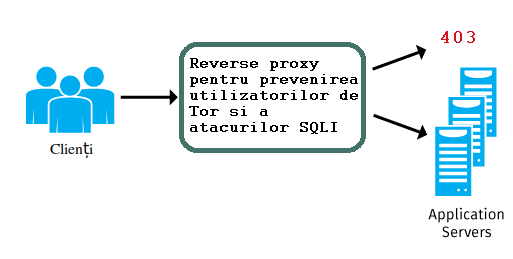
\includegraphics[width=0.6\textwidth]{fff.png}
	\caption{ Cutia neagră a sistemului.}
	\label{fig:black-box}
\end{figure}

Figura ~\ref{fig:black-box} prezintă cutia neagra a sistemului propus. \\

%\subsection{Functional Specification}
 \subsection{Specificații funcționale}

Sistemul trebui să prezinte o interfață grafică ușor de folosit de către utilizator și să fie capabil să redirecționeze traficul interceptat către un anumit server, clasificând și filtrând traficul malițios. Pentru a atinge obiectivele proiectului, următoarele cerințe funcționale trebuie îndeplinite: 
\begin{itemize}
  \item  Să realizeze conexiunea la un server HTTP/HTTPS și să redirecționeze traficul primit către acesta. 
  \item  Să intercepteze traficul venit pe o anumită interfață și port prestabilit. 
  \item  Să prelucreze request-urile primite de la clienți într-un format specific clasificatorului de SQL injection. 
  \item  Să nu redirecționeze reqest-urile clasificate ca și SQL injection. 
  \item  Să blocheze conectarea clienților ce folosesc IP-uri clasificate ca IP-uri de Tor. 
  \item  Să permită utilizatorului să editez și să vizualizeze lista IP-urilor de Tor. 
  \item  Să prezinte în interfața grafică toate intervențiile realizate asupra traficului(blocări de conexiuni sau de request-uri). 
  \item  Să permită utilizatorului să configureze modul de operare al sistemului. 
\end{itemize}


%\subsection{Non-Functional Specification}
 \subsection{Specificații non-funcționale}

Sistemul trebuie, de asemenea, să aibă următoarele caracteristici non-funcționale pentru a realiza obiectivele specificate: 
\begin{itemize}
  \item Să fie ușor de instalat și de folosit pentru orice utilizator, oricât de neexperimentat .
  \item  Să poată intercepta traficul de pe orice/oricâte interfețe disponibile. 
  \item  Să poată rula pe orice sistem de operare Windows cu Python2 instalat. 
  \item  Să aibă o rată de blocare de 100\% a IP-urilor de pe lista neagră, iar 
  în cazul detecției de SQL injection să nu aibă detecții false pozitive mai mari 2-3\% 
  și o acuratețe generală de peste 90\%.
\end{itemize}



